\documentclass[titlepage]{article}
\usepackage[utf8]{inputenc}
\usepackage[brazil]{babel}
\usepackage{parskip}
\usepackage{graphicx}
\usepackage{listings}
\graphicspath{ {images/} } 

\renewcommand{\lstlistingname}{Email}
\lstset{extendedchars=\true}
\lstset{inputencoding=ansinew}
\lstset{
  literate=
           {á}{{\'a}}1
           {ã}{{\~a}}1
           {à}{{\`a}}1
           {â}{{\^a}}1
           {é}{{\'e}}1
           {ê}{{\^e}}1
           {í}{{\'i}}1
           {ó}{{\'o}}1
           {õ}{{\~o}}1
           {ò}{{\`o}}1
           {ú}{{\'u}}1
           {ũ}{{\~u}}1
           {ç}{{\c{c}}}1
           {É}{{\'E}}1
           {Ó}{{\'O}}1
}

\title{Sugestões para reforma na biblioteca do IME-USP}
\author{Representantes de classe 2016 -- IME-USP}
\date{14 de setembro de 2016}

\begin{document}
\maketitle
\tableofcontents

\clearpage
\section{Introdução}
Este relatório apresenta ao diretor do IME-USP o resultado de diálogos entre 
representantes de classe do instituto sobre possíveis melhorias para a 
biblioteca. O intuito é colaborar para a construção de um ambiente capaz de
melhorar a experiência de ensino e aprendizagem.

O documento inicia-se com uma breve descrição do estado atual da biblioteca. 
Então, são apresentados os principais pontos levantados pelos representantes 
de classe, a saber, o objetivo contemporâneo da biblioteca no contexto 
universitário, a infraestrutura necessária para um estudo colaborativo, o 
papel de ferramentas tecnológicas e os serviços necessários para condução 
das atividades acadêmicas de ensino.

\subsection{Histórico}
No decorrer do primeiro semestre letivo de 2016, os representantes de classe
do IME se mobilizaram para oferecer um projeto mais completo para a biblioteca 
do instituto, após pedido do diretor. Nesse esforço, ocorreram extensivos 
diálogos, tanto em reuniões quanto por email, além de visitas à outras 
bibliotecas e uma consulta aberta à comunidade. Este relatório é fruto deste
trabalho.

\subsection{A biblioteca atualmente}
De acordo com o site institucional do IME-USP, a Biblioteca Professor Carlos
Benjamin de Lyra foi fundada em 1969 e possui um dos acervos mais completos na 
área de matemática da américa latina, além de um balcão de atendimento, armários
com chave para uso individual, salão de leitura com acomodação para 88 usuários,
3 salas especiais para estudo em grupo (de uso exclusivo dos alunos de 
graduação) e 6 salas para estudo individual (de uso exclusivo dos alunos de 
pós-graduação).

Na atual infraestrutura, são oferecidos pela biblioteca os seguintes serviços:
\begin{itemize}
\item Consulta e empréstimo, com prazo definido pela categoria do usuário.
\item Atualização do sistema de banco de dados bibliográficos DEDALUS.
\item Solicitação de cópias xerox através do sistema COMUT-ON LINE.
\item ARIEL --- sistema de transmissão de documentos on-line, entre as 
bibliotecas do SIBI-USP e outras universidades e instituições cadastradas 
no sistema.
\item Atendimento de empréstimo entre bibliotecas de todas as unidades da USP e
outras bibliotecas cadastradas.
\item Levantamentos bibliográficos, por meio de bases de dados nacionais e
internacionais.
\item Normalização técnica de documentos.
\item Orientação informal do usuário.
\item Treinamento na utilização do DEDALUS, e outras bases on-Line.
\item Solicitação de ISBN.
\item Elaboração de ficha catalográfica.
\item Intercâmbio de publicacões do IME-USP.
\item Registro e arquivamento da produção técnica e científica do IME-USP.
\item Murais informativos.
\end{itemize}

\clearpage
\section{Infraestrutura}

Há diversos comentários a serem feitos sobre aspectos físicos da biblioteca, que
podem ser resolvidos neste momento de mudança. 

\subsection{Iluminação Natural}
Acreditamos que essa é uma das chaves para um espaço de estudo mais convidativo,
e, consequentemente, melhor utilizado. Em todas as bibliotecas que visitamos, 
especialmente a da FEA --- observe a figura \ref{fig:luzfea} --- constatamos
a existência de grandes janelas e clarabóias, tanto nas salas de estudo quanto
no acervo. 

\begin{figure}[ht!]
\caption{Sala de estudos da biblioteca da FEA}
\label{fig:luzfea}
\centering
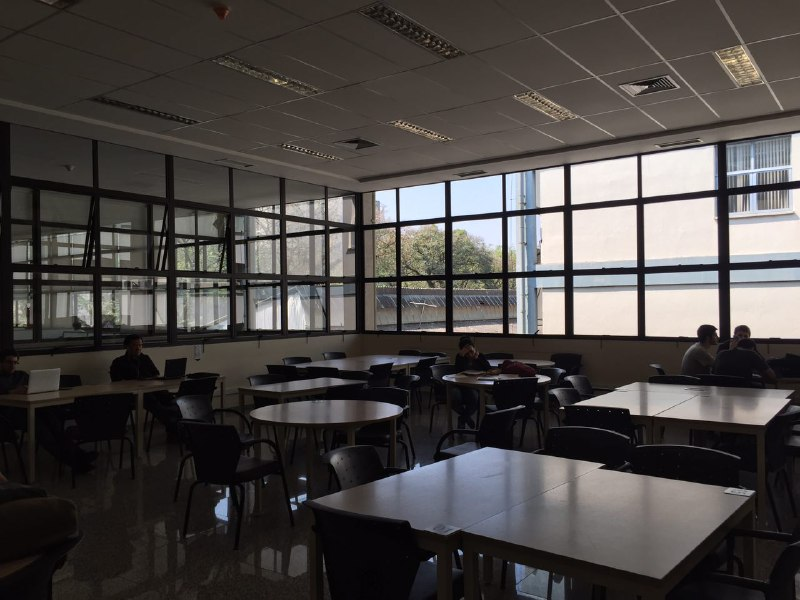
\includegraphics[width=1\textwidth]{fea-iluminacao}
\end{figure}

Isso torna o ambiente bastante iluminado e agradável. A biblioteca do IME, por 
seu próprio projeto, é bastante escura e isso se reflete na qualidade do 
ambiente. Acreditamos que não haja como abrir clarabóias no teto da biblioteca,
pois há andares do prédio por cima. Porém, outras medidas podem ser bastante 
efetivas, como a \emph{remoção ou troca das persianas das salas de estudo e no
acervo} (que ficam permanentemente fechadas), ou a \emph{abertura de  janelas 
grandes nas laterais do acervo}, onde há apenas janelas pequenas.

\subsection{Salas de estudo em grupo}
Uma dos principais problemas para os alunos do instuto é a dificuldade de
conseguir espaços para atividades de estudo em grupo. Isto faz com que muitos
vão estudar em outros lugares, em especial a FEA e a FAU, principalmente nas
semanas nas quais se concentram as avaliações.

Contudo, há a necessidade de espaço. Em uma visita à biblioteca, observou-se a 
existência de uma área grande e muito pouco utilizado entre o balcão dos 
funcionários e a entrada do acervo. Este local possui alguns sofás e estantes,
além de vários arquivos para indexação manual dos livros da biblioteca.  

Causa surpresa a existência de tal equipamento em pleno 2016, quando o sistema
DEDALUS cumpre este papel de forma muito mais eficiente e prática. De acordo 
com os funcionários da biblioteca, os arquivos classificados por autor e por 
título continuam sendo atualizados, enquanto os outros foram descontinuados.

Esse processo é custoso de diversas formas: mão de obra, espaço e oportunidade,
e o retorno é altamente questionável. Neste momento de escassez de recursos, 
há aqui uma clara oportunidade de melhoria na produtividade do instituto.

Tendo em vista o número insuficiente de salas para estudo em grupo na 
biblioteca, nossa sugestão é esvaziar este espaço (já que ele não é utilizado)
e utilizá-lo para construir quatro ou seis salas de estudo em grupo, como 
no esquema abaixo, onde na esquerda temos a situação atual com estantes e 
poltronas e na direita, a proposta de criação de novas salas.
\begin{figure}[ht!]
\caption{Organização atual e organização sugerida}
\label{fig:projeto}
\centering
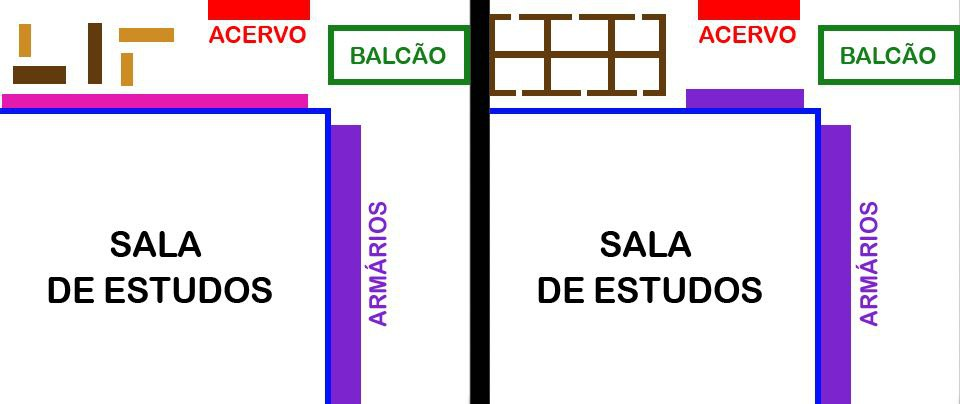
\includegraphics[width=1\textwidth]{projeto}
\end{figure}

\subsection{Tomadas}
Cada vez mais, ferramentas eletrônicas se tornam parte do processo de estudo dos
alunos. Os espaços que se sugerem a disponibilizar um ambiente propício a um 
estudo não podem mais ignorar este fato, e precisam estar adaptados a esta nova
realidade.

Infelizmente, na estrutura atual da biblioteca é complicado trabalhar com o
computador, ou com qualquer ferramenta eletrônica. Além de poucas tomadas,
estas estão mal posicionadas, e muitas vezes utilizá-las bloqueia o caminho dos
demais usuários do espaço. Mais ainda, no acervo o sinal da USPnet não é
confiável, deixando quem lá decide estudar sem acesso á internet.

Uma grande evidência de como a biblioteca atual peca neste aspecto é a 
quantidade de alunos que prefere estudar na rede linux, mesmo quando busca 
silêncio e utiliza seu notebook. Diversas vezes temos como resultado um espaço 
de estudo superlotado, enquanto outro é sub-utilizado.

Visitando a biblioteca da FEA, observamos que as salas de estudo em grupo de 
lá possuem mesas largas, com tomadas no centro --- observe a figura 
\ref{fig:tomada}. Sugerimos então a \emph{troca das mesas das salas por modelos
com tomadas embutidas}. 

\begin{figure}[ht!]
\caption{Tomadas nas mesas de estudo}
\label{fig:tomada}
\centering
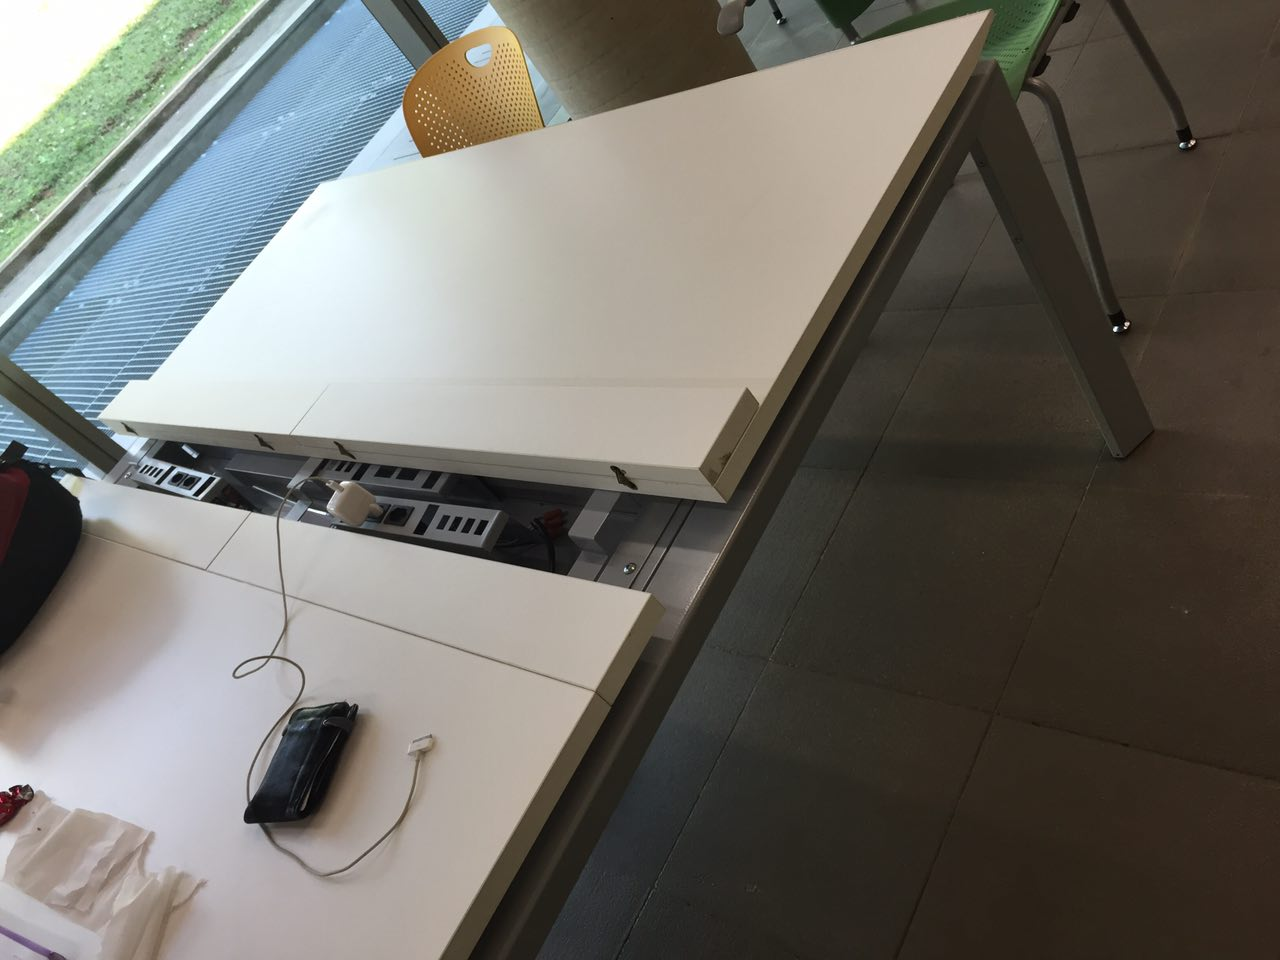
\includegraphics[width=1\textwidth]{tomada}
\end{figure}

\subsection{Recursos nas salas de estudo}
Além do espaço em si para possibilitar o estudo, é interessante que este esteja
equipado com o necessário para um trabalho produtivo.

Medidas interessantes nesta linha seriam a troca das cadeiras por modelos mais 
confortáveis e com rodas, a pintura das paredes com tons de branco, e a melhoria
na iluminação artificial. Lousas de canetão podem ser interessantes --- em 
locais com pouca circulação de ar é favorável evitar o pó do giz. Contudo, 
isso depende da disponibilidade de orçamento para comprar canetões, que são bem
mais caros que giz.

Também seria positivo a existência de projetores nas salas, ou a possibilidade 
de alugá-los direto no balcão, para proporcionar um ambiente para apresentações
ou reuniões entre alunos particpando de projetos que seja de mais fácil reserva
do que salas de aula.

\subsection{Sala de estudo individual}
Na sala de leitura, notamos a presença de algumas mesas grandes, possivelmente 
voltadas ao estudo em grupo. Como os alunos que utilizam esta sala valorizam o 
máximo de silêncio possível, é inviável utilizar estas para atividades em grupo.

Desse modo, elas se tornam um recurso ambíguo, e, por isso, mal utilizados. 
Assim, \emph{essas mesas poderiam ser retiradas para abrir espaço para mais 
cubículos}.  Na FEA, verificamos que também os cubículos \emph{possuem tomadas 
nas mesas}, para o uso de computadores.

\subsection{Acervo}
Algo que é único da nossa biblioteca é a presença de mesas de estudo dentro 
do acervo. Não encontramos esse padrão em nenhum outro local visitado. 

Percebemos que esta característica é algo importante para os alunos, que gostam 
de estudar perto dos livros, seja pelo silêncio, seja pelo acesso rápido aos
títulos. Por isso, uma sugestão seria, \emph{proporcionar mais mesas mesas e 
mesas melhores}, tanto com tomadas quanto com iluminação própria.

Foi dito para nós pelos funcionários da biblioteca que as salas na lateral do 
acervo estão sendo desocupadas e serão retiradas dali. Ao discutir usos para o 
espaço, ponderamos que talvez não haja necessidade de mais salas para grupos 
ali, dado as salas existentes mais as novas anteriormente sugeridas.

Seria portanto interessante utilizar este local para reorganizar as estantes e 
mesas, deixando o acervo menos apertado e abrindo espaço para mais mesas de 
estudo, que se aproveitariam também das grandes janelas da lateral, com melhor
iluminação natural.

A organização do acervo também é um ponto muito importante. Na FEA, as 
estantes são maiores e mais robustas, e possuem um diferencial muito 
importante: possuem cores nas laterais identificando o que há nelas: se são 
livros, periódicos, teses (figura \ref{fig:cores}). 

\begin{figure}[ht!]
\caption{Estantes de livros na FEA}
\label{fig:cores}
\centering
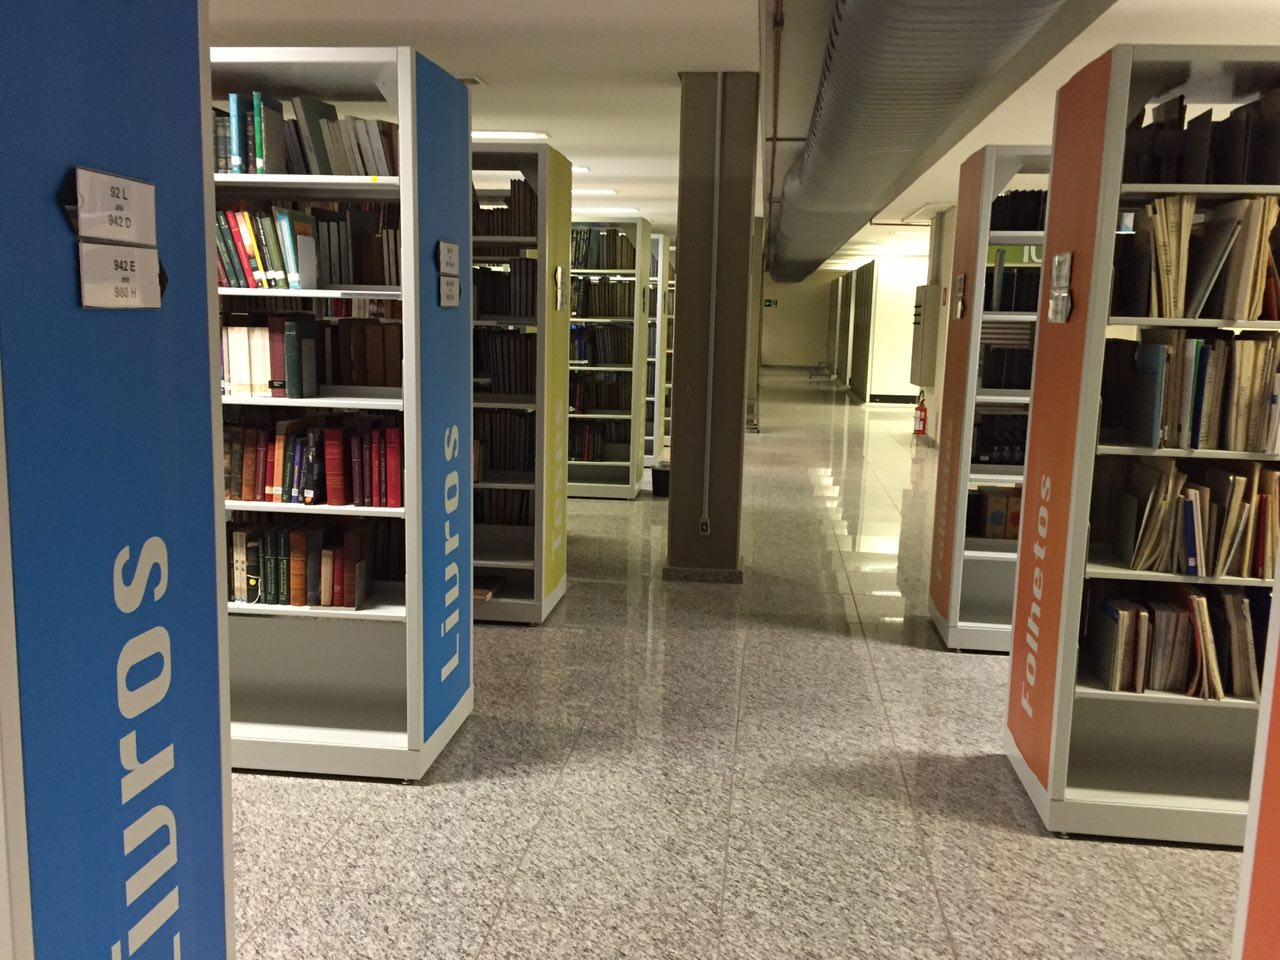
\includegraphics[width=1\textwidth]{cores}
\end{figure}

A mesma abordagem poderia ser utilizada no IME, utilizando cores para 
identificar as estantes com livros de seções ou cursos distintos. Com o auxílio
visual, a localização das obras se torna muito mais prática, especialmente para 
quem não utiliza muito a biblioteca. Na mesma linha, um mapa pode ser colocado 
na parede próxima à entrada do acervo, mostrando a disposição das estantes de 
cada cor/tema no espaço da biblioteca.  

\clearpage
\section{Serviços}
Além de sugestões para a organização física da biblioteca, também coletamos 
sugestões para a organização dos serviços prestados por essa.

\subsection{Armários}
Os armários da biblioteca são um pouco apertados para quem carrega bolsas 
grandes, que costuma ser o caso dos estudantes que moram longe e passam o dia
na universidade. Na FEA, vimos \emph{armários metálicos bem espaçosos} (figura 
\ref{fig:armario}). 

\begin{figure}[ht!]
\caption{Ármarios da FEA}
\label{fig:armario}
\centering
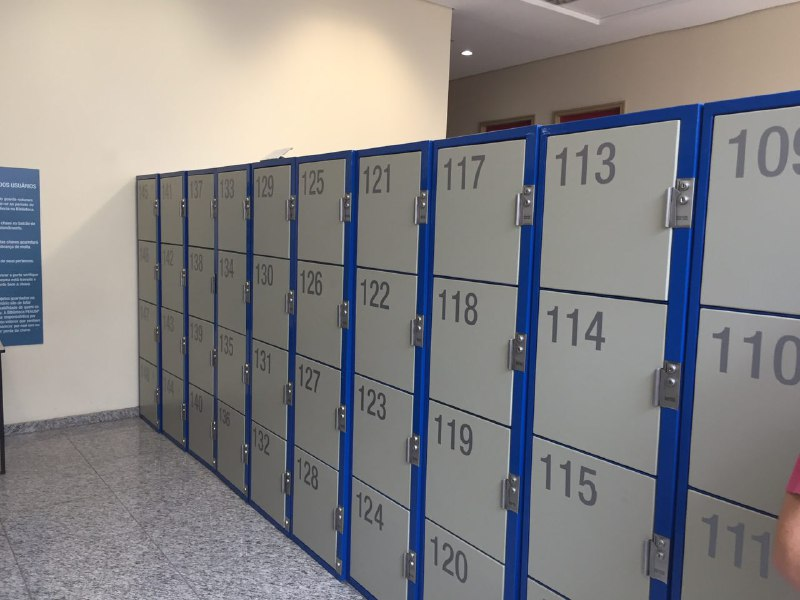
\includegraphics[width=1\textwidth]{armario}
\end{figure}

Nossa sugestão é, portanto, trocar os armários por esses modelos. Isso 
reduziria o número de armários, o que talvez seja problemático. Uma solução 
seria \emph{colocá-los após o balcão, onde agora estão os arquivos de indexação 
do acervo}.

Outra sugestão é a utilização de cordinhas de plástico para segurar as chaves 
do armário ao invés dos barbantes atuais, tanto por motivos de higiêne quanto
para obter maior durabilidade.

Na nossa biblioteca, ao se pedir um armário, o cartão USP do usuário fica retido
com o balconista. Em outras, o cartão é apenas escaneado com um leitor de código
de barras. De acordo com os funcionários, este cuidado extra ocorre devido ao 
número de pessoas que utilizam o armário para outros fins que não o uso da 
biblioteca --- por exemplo, guardar seus pertences ali para ir almoçar. 

Os funcionários nos disseram que não é um número tão grande de pessoas a ponto 
de ameaçar a disponibilidade de armários, mas isto poderia mudar caso o 
documento não ficasse retido.

Ainda assim, trata-se de uma inconveniência, e poderia ser feito um teste de 
alguns dias para avaliar o impacto. De qualquer modo, isso reflete um problema
externo à biblioteca, que é a falta de armários para uso geral pelos alunos. 

\subsection{Reserva de salas}
Poder reservar as salas de estudo em grupo por um horário fixo seria muito 
conveniente. Atualmente as (poucas) salas são de quem chegar primeiro, pelo 
tempo que quiser.

Essa reserva poderia ser feita utilizando uma simples agenda de papel, 
controlada pelos funcionários da biblioteca. Seria apenas necessário pensar em
regras para evitar o abuso deste recurso; principalmente evitar que alguém 
reserve uma sala por muitas horas ou que reserve e não compareça.

Bons critérios para resolver este problema poderiam amenizar a falta de espaços
de estudo em grupo, de forma bem barata. Junto da criação dos novos espaços,
torna-se possível atender com maior qualidade à demanda do instituto.

\subsection{Devolução de livros}
\begin{figure}[ht!]
\caption{Caixa para devolução rápida de livros}
\label{fig:caixa}
\centering
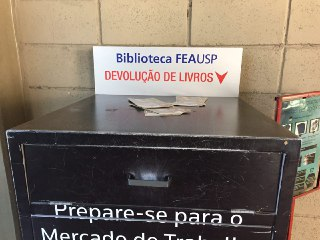
\includegraphics[width=1\textwidth]{caixa}
\end{figure}

Na FEA vimos a caixa da figura \ref{fig:caixa} para devolução rápida de livros.
É algo bastante prático, principalmente por ampliar o horário de devolução das
obras.

Dois lugares interessantes para colocar seriam a porta da biblioteca, ao lado 
dos murais, e algum ponto no bloco B.

Contudo, esta iniciativa geraria mais trabalho para o pessoal da biblioteca,
sendo restringida pela disponibilidade de algum funcionário ir lá buscar os 
livros de tempos em tempos. Dependendo da situação de pessoal, isto pode ser
problemático.

Também ficamos um pouco em dúvida se jogar o livro na caixa não poderia 
danificar ele, e se há alguma regra ou restrição para isto. Contudo, não 
conseguimos descobrir uma resposta para isso.

\subsection{Internet}
A qualidade do acesso à internet na biblioteca é péssima. Dentro do acervo, não
há sinal de 3G e nem Wi-Fi, e na sala de estudos o Wi-Fi não dá conta do 
número de pessoas.

Para encaminhar este problema, sugerimos espalhar mais roteadores pelos vários 
espaços da biblioteca. Uma restrição é a qualidade ruim da rede USPNet, que 
faz com que vários institutos tenham suas próprias redes (Feanet, Polinet), 
refletindo tanto a necessidade de acesso. Mais ainda, esta não é uma questão
específica da biblioteca, mas um problema do instituto como um todo.

\subsection{Sistemas}
Na biblioteca Brasiliana, nos deparamos com estes suportes --- figura 
\ref{fig:qr} -- que disponibilizam QR Codes dos principais sistemas da USP, para 
consulta rápida. Achamos isto uma comodidade bem interessante, além de ser algo
simples e barato de disponibilizar.

\begin{figure}[ht!]
\caption{QR codes promovendo serviços da biblioteca}
\label{fig:qr}
\centering
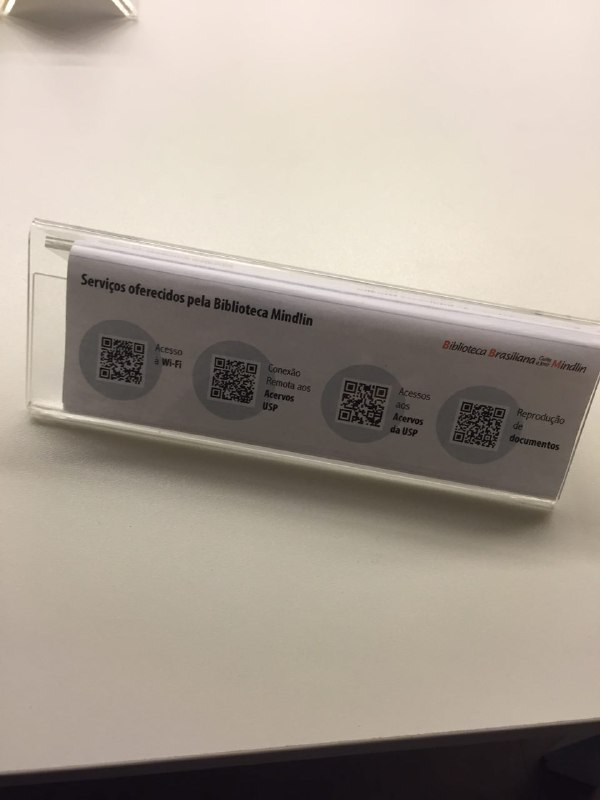
\includegraphics[width=.6\textwidth]{qr}
\end{figure}

\subsection{Salas específicas para pós graduação e graduação}
Dado as restrições de espaço e a grande demanda dos alunos por locais de estudo,
parece proveitoso retirar a restrição de pós-graduação e graduação, apenas
organizando melhor o uso destes ambientes.

Se de fato for interesse privilegiar os alunos de mestrado e doutorado nesta
questão, bastaria então fazer com que o critério de reserva destes locais, mesmo
que aberto à todos, dê maior prioridade para eles.

\clearpage
\section{Emails enviados pelos representantes de classe}

\begin{lstlisting}[caption=Enviado por Nathan Proença]
Bom dia, pessoal

Estou mandando esse email para a lista para levantar 
sugestões para o projeto de biblioteca do IME. Por favor 
respondam com sugestões para a gente mandar para a 
diretoria sobre uma possível reforma da biblioteca. Na 
primeira reunião dos RC's de 2016, o Giuliano levantou 
esse ponto, e disse que o Clodoaldo pediu ideias nossas .  

Meus comentários:
As salas de estudo em grupo são ótimas, o principal 
problema sendo que são poucas. Em época de avaliação, é 
bem complicado conseguir uma. Se possível, quanto mais 
delas, melhor seria. Ainda assim, tem dois aspectos sobre 
essas salas que eu vejo que poderiam ser melhor: Poderiam 
ter um melhor isolamento acústico entre as salas, e 
poderia haver mais tomadas e em melhores condições, para 
facilitar o uso de computadores.

A sala de leitura é claramente um espaço bem aproveitado 
e sempre tem bastante gente usando para estudar. Ainda 
assim, a locomoção entre os cubículos é complicada, e há 
apenas 2 ou 3 tomadas, concentradas num lado da sala. Em 
geral por causa disso, quando preciso trabalhar com meu 
computador num espaço silencioso, acabo optando pela rede 
linux ou pelo CCSL.

Enfim, tldr: Mais lousas, tomadas e espaços de estudo em 
grupo.
\end{lstlisting}

\begin{lstlisting}[caption=Enviado por Jackson Souza]
As lousas atuais são boas? Ou seja, dá pra escrever nelas 
e apagar com facilidade? 

Se alguém conseguir enxergar que o uso de projetores 
seria útil também vale sugerir. Se for possível viajar 
um pouco poderia ser bem interessante escrever nas 
paredes se elas fossem pintadas com tinta e fosse usado 
um giz/canetão especiais, claro.
\end{lstlisting} 

\begin{lstlisting}[caption=Enviado por Gustavo Estrela]
Acho que o problema da falta de salas de grupo podia ser 
amenizado se tivesse um sistema de reserva das salas. Do 
jeito que está agora a sala é de quem chegar primeiro até 
a pessoa decidir sair, não é?
\end{lstlisting}

\begin{lstlisting}[caption=Enviado por Gustavo Silva]
Acho que as salas poderiam ser mais apropriadas pra 
estudos com computador. Ter mais tomadas, rede sem fio (a 
USPnet não pega na parte de dentro da biblioteca, nas 
salas eu nunca testei), um projetor para ligar o notebook
. Isso faria pessoas que lotam a sala BCC em época de EPs 
migrar para essas salas. E se não me engano as lousas são 
de giz, seria bem melhor mudar pra lousa de canetão.
\end{lstlisting}

\begin{lstlisting}[caption=Enviado por Carlos E. Ferreira]
Acho que vocês têm de pensar no que mais faz falta na 
biblioteca. Eu tenho a sensação, que faz falta espaço de 
estudo de todos os tipos: 

- individual de boa qualidade, com espaço para você 
colocar seu computador, ter acesso à rede de boa qualidade,
estudar, fazer seus trabalhos, etc. 
- de pequenos grupos (2 pessoas) onde possa discutir com 
um colega, trabalhar junto, etc com espaço pro computador
, rede, etc. 
- grupos maiores, aqui sim com lousa, eventualmente 
projetor, espaço de computador, etc. 

Pelo que lembro, temos 2 salas de estudo em grupo, 8 
salas de estudo pequenas (que só a pós pode usar), e o 
salão com aquelas mesas pequenas. O espaço do acervo me 
parece subutilizado. E quando você passeia por ele e vê 
os títulos dos livros nas estantes, têm certeza de que 
muito do que está ali poderia ser removido sem nenhum 
prejuízo (livros de clipper, MSDOS, Wordstar e por aí vai
). Seria legal pensar o que precisamos manter no acervo, 
e que ambiente seria legal manter lá prá conseguir 
maximizar o espaço dedicado a estudos. 

Não consigo entender por que alguém prefere lousa branca 
a lousa de giz, mas tudo bem, vocês que mandam. Gosto 
muito da ideia da parede que servisse de "lousa". Alguém 
já sugeriu isso pro CCSL? Seria bacana ver as pessoas 
trabalhando em todos os corredores.
\end{lstlisting}


\begin{lstlisting}[caption=Enviado por Renato Cordeiro]
Essa questão de espaço, para falar a verdade, é um 
problema geral do instituto. Os tópicos levantados pelo 
Carlinhos resumem bem os três tipos de locais que nós 
precisamos. Talvez não dê para resolver tudo dentro da 
biblioteca, mas se repassarmos para o diretor a 
necessidade desses espaços, podemos manter em discussão a 
criação de novas áreas para estudo.

Se bem me lembro, dentro da biblioteca existe um pequeno "
espaço de leitura", logo antes do acervo e ao lado da 
recepção, com um banco ou sofá, duas prateleiras com os 
livros novos do mês e jornais. Alguém usa aquele espaço? 
Porque nas poucas vezes que eu entrei na biblioteca, 
raramente vi alguém parado por lá. Lá dentro também 
existem uns 5 ou 6 computadores, que as pessoas usam para 
consultar o Dedalus. Será que eles são realmente 
necessários? As pessoas podem ir com os livros anotados 
num papel, usar o celular, etc. Acho que a maioria das 
pessoas deixa para consultar o código dos livros lá só 
porque sabem que tem computadores. Eu economizaria esse 
espaço (e até o custo de manter aqueles PCs) para 
aumentar o espaço para os alunos.

Concordo com a ideia de um sistema de reserva para as 
salas de estudo. Não precisa ser nada tecnológico: uma 
folha de sulfite para reservar um horário na semana é 
suficiente. Melhor que uma solução online, inclusive: 
evita reservas à toa, estimula o planejamento e diminui o 
desperdício de tempo lá dentro (se você tem 2h, é melhor 
usá-las bem. Por não ter um prazo para sair, muita gente 
acaba procrastinando lá dentro, e desperdiçando tempo que 
poderia ser útil para outros).

Acho que a proposta daquelas mesas maiores da sala de 
estudo era criar esse "espaço para pequenos grupos" que o 
Carlinhos comentou. Só tem um problema: como não existe 
divisão para as áreas com mesas individuais, as pessoas 
acham ruim se você se sentar em 2 ou 3 pessoas e começar 
a conversar. Me lembro de ter sentado uma vez para 
resolver uma lista de exercício com dois colegas, começar 
a falar sobre ela e, em algum momento, uma pessoa chegar 
até nós e pedir para fazermos silêncio. Acho que muita 
gente não usa aquela área por causa dessa "lei do silêncio
" culturalmente imposta. É claro que isso é útil para 
leitura, por exemplo. Mas também faz daquele lugar uma 
área em que as pessoas vão para dormir... Eu ressaltaria 
para o diretor que esse espaço de pequenos grupos deveria 
ser separado do individual. Assim, quem precisar falar 
pode usar uma área sem problemas. Quem quiser silêncio, 
também terá sua necessidade respeitada.

Como não existe verba para que essa reforma seja feita "
agora", não seria possível melhorar alguns aspectos mais 
rapidamente? Por exemplo: se o wifi nas salinhas é ruim, 
não é possível instalar mais um acess point lá dentro? O 
Will e o pessoal da rede IME podem dizer se isso é viável 
ou não. Se for de comum acordo entre os alunos, será que 
podemos instituir esse sistema de reservas? Pela minha 
proposta, precisamos apenas de um calendário em papel (ou 
uma agenda, como a da sala de reuniões do Bloco C). 
Ficaria registrado, inclusive, quem usou a sala e quando (
se acontecer algum problema).

Para terminar (já escrevi muito), acho que o IME deveria 
pensar em espaços mais dinâmicos: como o Carlinhos disse, 
o espaço deve atender às nossas necessidades, mas 
necessidades mudam com o tempo. Se tudo no IME for sempre 
100% construído para atender a um público X de uma dada 
época, o instituto estará sempre desatualizado. Afinal, 
hoje estamos coletando propostas que poderão ser 
implementadas só daqui a uns 5 anos - quando quase nenhum 
de nós estará mais no instituto. Será que a necessidade 
das pessoas em 202X será a mesma da nossa? Se pararmos 
com essa rigidez e permitirmos espaços mais abertos, que 
possam ser rearrumados, economizaremos muito tempo e 
dinheiro no futuro. E como eu aplicaria isso na 
construção da biblioteca? Primeiro, vamos parar de 
assumir que as salas não devem ter tomadas: cada vez mais 
pessoas usam computadores, isso é uma realidade e devemos 
dar condições de que as pessoas estudem com seus notebooks.
Também acho que as tomadas deveriam ficar melhor 
espalhadas. Não precisamos ser overkill na estrutura, mas 
distribuir a energia elétrica uniformemente pelas paredes 
e pelo meio da sala (no chão?) permitiria que mudássemos 
a conformação do espaço sem ter de destruir a sala e 
refazê- la.

TL;DR: a sala de leitura até tem um espaço para estudo em 
grupo (mesas grandes), mas a "lei do silêncio" que existe 
lá não deixa ninguém usá-lo como tal; reserva de salas é 
uma boa, e wi-fi também - não podemos tentar resolver 
isso antes da reforma? O espaço de estudo deveria ser 
mais dinâmico (permitir que ele seja rearrumado no futuro 
sem reformas): as necessidades dos alunos de hoje não são 
as mesmas dos alunos do futuro, e construir baseado nisso 
pode economizar tempo e dinheiro.
\end{lstlisting}


\begin{lstlisting}[caption=Enviado por Aurea Hariki]
Oi,

Não sou nem do BCC mas vou dar minha opinião mesmo 
assim.

Na biblioteca do meu antigo colégio tinha um espaço de 
estudos com várias mesas, computadores, três salas de 
estudo em grupo (2 salas para grupos de 5  pessoas e uma 
sala para 9) todas com um computador e quadro branco; e 
três salas de estudo em dupla com um computador. As 
reservas das salas e das mesas eram feitas online e era 
ótimo, mas tinha o problema de reservarem a sala e não 
usarem e também reclamações do barulho. Podiam colocar 
uma tolerância,  por exemplo, se você reservou pra 13h e 
não chegou até 14h perdeu o horário e agora a sala é open 
pra quem chegar. Ou então deixar usarem até quem reservou 
chegar. Podiam colocar um limite de tempo de reserva 
também, tipo não deixar a mesma pessoa reservar 10 horas 
seguidas.

No sistema de reserva da minha escola era preciso 
identificar cada uma das pessoas que usaria aquele espaço
, então a gente precisava de muito planejamento. Não sei 
se tanta rigidez é necessária no ambiente universitário, 
então o esquema de só uma pessoa responsável reservar, 
mas quando for usar tem que ter uma quantidade 
considerável de pessoas para usar as salinhas ainda 
parece dar certo.

Gosto muito das salinhas de estudos e super apoio 
construirem mais, mas não gostaria que reduzissem o 
espaço da sala de leitura para isso.

A falta de tomadas e acesso à Internet é realmente um 
problema, mas como eu sou da pura, consigo facilmente me 
virar sem isso (não sou capaz de opinar).

Gosto dos computadores dentro do acervo para consultar o 
dedalus e não vi muito motivo para tirar. Falar que podem 
olhar antes ou olhar no celular só dificultaria o uso da 
biblioteca. 

A sala de leitura também é muito boa e está sempre cheia (
mas não lotada), o que é ótimo. Eu, pessoalmente, me 
sinto muito desconfortável naquele ambiente porque não se 
pode fazer barulho nenhum. Muitas pessoas gostam do 
silêncio que é lá e eu não quero atrapalhar, então nem 
entro.

Alternativamente, para estudar sozinha, eu uso a rede 
linux ou Rede IME mesmo que não precise usar os 
computadores só porque é menos tenso. Por outro lado, as 
mesas de estudo com tomadas e sem computadores geralmente 
estão cheias também, então eu acabo pegando um computador 
que outra pessoa podia estar querendo e eu nem precisava 
tanto.

As mesas azuis também são muito boas, tirando o calor e a 
falta de tomadas. É o melhor espaço que temos pra 
realmente discutir ideias sem nos preocuparmos em 
atrapalhar o silêncio dos outros. O problema é que são 
poucas mesas e estão sempre cheias (muitas vezes sendo 
usadas por pessoas jogando baralho, mas ok). Acho que 
seria bom ampliar o espaço das mesas azuis (talvez até 
tirar as plantas na frente da sessão de alunos para ter 
mais espaço).

(Tl;dr. Reserva de salas? Ótimo, só não vamos deixar as 
salas vazias por 4h ou deixar a mesma pessoa com uma sala 
por 10h.  Sala de leitura me deixa ansiosa, uso a Rede 
IME Mesas azuis: Quero mais.)
\end{lstlisting}


\begin{lstlisting}[caption=Enviado por Renato Cordeiro]
Só reiterando as ideias da Aurea:

    Em 21 de março de 2016 16:34, Aurea Hariki 
    <aureahariki@gmail.com> escreveu:
    Oi,
    Não sou nem do BCC mas vou dar minha opinião mesmo 
    assim.

Não é problema nenhum você opinar, é claro. Ter a opinião 
de todos os cursos é essencial, dado que o espaço é de 
todos nós e cada um pode ter usos ligeiramente 
diferentes.

    Na biblioteca do meu antigo colégio tinha um espaço de 
    estudos com várias mesas, computadores, três salas de 
    estudo em grupo (2 salas para grupos de 5  pessoas e uma 
    sala para 9) todas com um computador e quadro branco; e 
    três salas de estudo em dupla com um computador. As 
    reservas das salas e das mesas eram feitas online e era 
    ótimo, mas tinha o problema de reservarem a sala e não 
    usarem e também reclamações do barulho. Podiam colocar 
    uma tolerância,  por exemplo, se você reservou pra 13h e 
    não chegou até 14h perdeu o horário e agora a sala é open 
    pra quem chegar. Ou então deixar usarem até quem reservou 
    chegar. Podiam colocar um limite de tempo de reserva 
    também, tipo não deixar a mesma pessoa reservar 10 horas 
    seguidas.

Acho que um tempo limite é necessário. Só não tenho 
certeza de quantas horas poderia ser. Talvez 6h? Menos? 
Acho que reservar durante um período do dia ~4h é 
bastante tempo, e a maioria das pessoas para de se 
concentrar (principalmente em grupo) quando fica muito 
tempo no mesmo assunto. Um limite reduziria tanto a 
monopolização quanto o "mal aproveitamento" do tempo da 
sala. 

    No sistema de reserva da minha escola era preciso 
    identificar cada uma das pessoas que usaria aquele espaço
    , então a gente precisava de muito planejamento. Não sei 
    se tanta rigidez é necessária no ambiente universitário, 
    então o esquema de só uma pessoa responsável reservar, 
    mas quando for usar tem que ter uma quantidade 
    considerável de pessoas para usar as salinhas ainda 
    parece dar certo.

Rigidez em excesso só tende a complicar as coisas, 
realmente. Reservar no nome de uma pessoa, mas exigir que 
ela entre na sala com um mínimo de pessoas parece hiper 
razoável.

    Gosto muito das salinhas de estudos e super apoio 
    construirem mais, mas não gostaria que reduzissem o 
    espaço da sala de leitura para isso.
    A falta de tomadas e acesso à Internet é realmente 
    um problema, mas como eu sou da pura, consigo facilmente 
    me virar sem isso (não sou capaz de opinar).
    Gosto dos computadores dentro do acervo para consultar o 
    dedalus e não vi muito motivo para tirar. Falar que podem 
    olhar antes ou olhar no celular só dificultaria o uso da 
    biblioteca. 

No fundo, os computadores não atrapalham muito. Eu sugeri 
que eles poderiam ser retirados para não ocupares espaço 
em excesso. Talvez posicioná-los em outro local (
espalhados no meio do acervo?) fosse até mais prático.  

    A sala de leitura também é muito boa e está sempre cheia (
    mas não lotada), o que é ótimo. Eu, pessoalmente, me 
    sinto muito desconfortável naquele ambiente porque não se 
    pode fazer barulho nenhum. Muitas pessoas gostam do 
    silêncio que é lá e eu não quero atrapalhar, então nem 
    entro.

Pelo que ouvi de pessoas de outros institutos, parece que 
essa "lei do silêncio" é bem característica do IME. 
Especificamente, já vi conhecidos da FFLCH falarem que 
preferem vir ler no IME porque nós fazemos mais silêncio 
que nas áreas de estudo e dentro da biblioteca 
deles.

    Alternativamente, para estudar sozinha, eu uso a rede 
    linux ou Rede IME mesmo que não precise usar os 
    computadores só porque é menos tenso. Por outro lado, as 
    mesas de estudo com tomadas e sem computadores geralmente 
    estão cheias também, então eu acabo pegando um computador 
    que outra pessoa podia estar querendo e eu nem precisava 
    tanto.

Vejo muita gente fazendo isso. Por isso, acho que 
poderíamos dividir o espaço da sala de estudo em dois: um 
para estudo individual, sendo a "área silenciosa" e outro 
para estudo mais geral. Assim, talvez, as pessoas 
poderiam aproveitar melhor aquele espaço para 
conversar.

    As mesas azuis também são muito boas, tirando o calor e a 
    falta de tomadas. É o melhor espaço que temos pra 
    realmente discutir ideias sem nos preocuparmos em 
    atrapalhar o silêncio dos outros. O problema é que são 
    poucas mesas e estão sempre cheias (muitas vezes sendo 
    usadas por pessoas jogando baralho, mas ok). Acho que 
    seria bom ampliar o espaço das mesas azuis (talvez até 
    tirar as plantas na frente da sessão de alunos para ter 
    mais espaço).

As mesas azuis são muito boas, realmente. Só uma delas 
fica do lado de uma lousa, e eu sempre achei que 
poderíamos colocar pelo menos mais uma lousa do lado da 
B10. Como o IME tem poucos espaços para a graduação, o 
pessoal acaba usando as mesmas áreas para várias 
atividades (jogar baralho inclusive). Na maior parte do 
tempo, quando tem poucas pessoas, isso não atrapalha. Mas 
nas épocas mais agitadas - de listas e provas - é bem ruim
...

Se não me engano, uma parte da área da nova lanchonete 
terá mesas para as pessoas usarem. Se for verdade, isso 
deve ajudar a "desafogar" as mesas azuis.

Reitero que seria bom levar todos esses pontos para o 
diretor, dado que ele nos deu a abertura para tal. Se a 
reforma da biblioteca demorar, pode ser que consigamos 
melhorar algumas coisas em menos prazo, com pouco ou 
nenhum custo. De outro modo, abrimos a discussão sobre a 
melhora de outros espaços do instituto.
\end{lstlisting}


\begin{lstlisting}[caption=Enviado por Giuliano Salcas Olguin]
Pessoal,

gostaria de contribuir com alguns exemplos.

De Harvard, tem um serviço interessante de digitalização 
de páginas de livros, em: http://library.harvard.edu/get-
it-services. Aliás, isso estão na missão deles, em : http
://library.harvard.edu/09222015-0951/strategic-priorities-
fy16

Sobre os locais de estudos, em Stanford, http://library.
stanford.edu/#middle-tab-240, existem diferentes 
modalidades de espaços. Em uma delas, em particular:

Seven study rooms, each with space for groups of up to 
six people, are available outside the main reading rooms 
in the Bing Wing. Most rooms are equipped with white 
boards, and one (outside the Jonsson Social Science 
Reading Room) has a smart board as well.

Policies:
Rooms are available on a first-come basis
Groups of two or more take priority over single-person use
Observe a two-hour limit when others are waiting
No food or drinks

Outra é 24 horas!
The 24-hour study room has dual-boot Mac/Windows computers
, laptop-support displays, and large tables for quiet 
individual study. A valid Stanford ID Card is required 
for entry.

abs,
\end{lstlisting}

\begin{lstlisting}[caption=Enviado por Victor Sprengel]
Olá,
Tentarei complementar a discussão e evitar opiniões que 
simplesmente concordam com o que ja foi dito. Estou 
gostando da discussão de modo geral.

Eu pessoalmente não gosto de reservas. Sinto como se elas 
fossem um 'band-aid fix' para um espaço que está sempre 
ocupado e logo é necessário competir por ele. Com o 
sistema de reserva, quando a decisão de estudar em grupo 
é repentina, ela também torna-se quase sempre inviável. 

A pós costuma usar as salas de estudo da biblioteca 
designadas para eles? As poucas pessoas que conheço da 
pós parecem preferir muito mais a leitura individual. 
Talvez não fosse um problema compartilhar aquelas salas, 
desde que haja algum tipo de prioridade.

Como Carlinhos mencionou, o acervo poderia se livrar de 
parte de sua coleção que já não faz mais sentido. 
Eventualmente até vender esses livros num feirão para 
arrecadar dinheiro para a reforma? Lá é um bom espaço 
para mesas de estudo silencioso / uso de notebook. Na 
FFLCH acontece algo parecido.

Como anda o processo da lanchonete no bloco B? Uma das 
propagandas que ouvi de lá é justamente um local para 
estudo. Vale a pena comentar algo sobre isso nesse 
documento sobre bibliotecas ?

Sei que isso envolve questões de seguranças, mas um 
defeito das mesas azuis é que lá é uma estufa no verão. 
Não poderiamos negociar de deixar a porta aberta para 
ventilar ar? Ou propor alguma solução alternativa? (
ventiladores ?)

Faltam cadeiras nas mesas azuis. Algumas das (já 
insuficientes) que estão lá também estão quebradas. 
Tomadas também.

Gosto de tempo limite para salas de estudo em dupla e 
grupo e acho que substitui a reserva.

Bem, esses são os pontos que eu gostaria de levantar, 
considerem apenas os que de fato são pertinentes para a 
discussão (posso ter divagado um pouco). Eu dei uma 
rápida revisada no texto e alterei um pouco a seção 
INFRAESTRUTURA pois achei que estava muito enxuta. Assim 
que existir uma noção mais concreta do que precisa estar 
no documento, eu posso redigir bastante coisa.

Abraços,
\end{lstlisting}


\begin{lstlisting}[caption=Enviado por Leonardo Lana]
Olá,

Os funcionários da biblioteca queixaram-se sobre falta de 
acessibilidade do balcão, devido à sua altura; e a falta 
de uma brigada de incêndio próxima ao acervo.

Eles sugeriram que as salas no fundo do acervo, as quais 
estão sendo usadas para guardas materiais para a reforma, 
entre outras coisas, sejam transformadas em salas de 
estudos em grupo pós reforma.

Abraços,
\end{lstlisting}

\end{document}
